% Standalone TikZ source for the EDMA block diagram (Fig. 1).
% Compile: latexmk -pdf block_diagram_src.tex; copy PDF to block_diagram.pdf
\documentclass[tikz,border=2pt]{standalone}
\usepackage{amsmath,amssymb,bm}
\newcommand{\mb}[1]{\mathbf{#1}}
\usetikzlibrary{arrows.meta,positioning,fit,calc}
\begin{document}
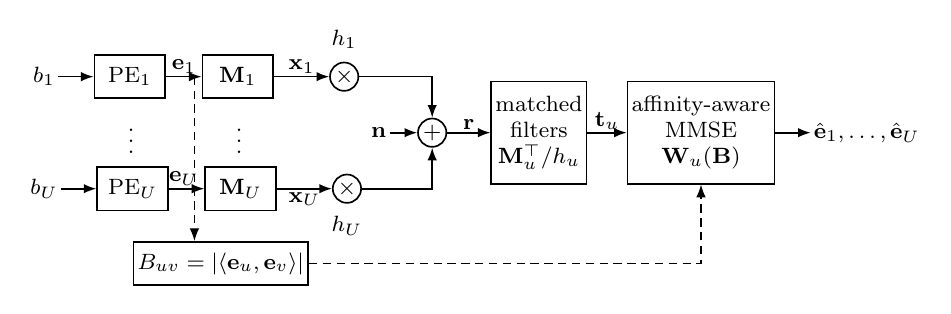
\begin{tikzpicture}[
  font=\footnotesize,
  node distance=3.2mm and 4.5mm,
  blk/.style={draw, semithick, minimum height=5.5mm, minimum width=9mm,
              inner sep=1.5pt, align=center},
  sum/.style={draw, semithick, circle, inner sep=0pt, minimum size=3.6mm},
  arr/.style={-{Latex[length=1.6mm]}, semithick},
  dsh/.style={-{Latex[length=1.6mm]}, densely dashed, thin},
  lbl/.style={inner sep=1pt}
]
% ---------------- user 1 chain ----------------
\node[lbl] (b1) {$b_1$};
\node[blk, right=of b1] (pe1) {$\mathrm{PE}_1$};
\node[blk, right=of pe1] (m1) {$\mb{M}_1$};
\node[sum, right=7mm of m1] (h1) {$\times$};
\node[lbl, above=1.2mm of h1] {$h_1$};
% ---------------- user U chain ----------------
\node[lbl, below=11mm of b1] (bU) {$b_U$};
\node[blk, right=of bU] (peU) {$\mathrm{PE}_U$};
\node[blk, right=of peU] (mU) {$\mb{M}_U$};
\node[sum, right=7mm of mU] (hU) {$\times$};
\node[lbl, below=1.2mm of hU] {$h_U$};
% vdots between chains
\path (pe1) -- (peU) node[midway] {$\vdots$};
\path (m1) -- (mU) node[midway] {$\vdots$};
% ---------------- channel sum ----------------
\path (h1) -- (hU) node[midway] (mid) {};
\node[sum] (sig) at ($(h1)!0.5!(hU)+(11mm,0)$) {$+$};
\node[lbl, left=3.5mm of sig] (nn) {$\mb{n}$};
% ---------------- receiver ----------------
\node[blk, right=5.5mm of sig, minimum height=13mm] (mf)
  {matched\\ filters\\ $\mb{M}_u^{\top}/h_u$};
\node[blk, right=5mm of mf, minimum height=13mm] (wnr)
  {affinity-aware\\ MMSE\\ $\mb{W}_u(\mb{B})$};
\node[lbl, right=4.5mm of wnr] (out) {$\hat{\mb{e}}_1,\ldots,\hat{\mb{e}}_U$};
% ---------------- affinity measurement ----------------
\coordinate (tap1) at ($(pe1.east)!0.8!(m1.west)$);
\coordinate (tapU) at ($(peU.east)!0.8!(mU.west)$);
\node[blk] (bm) at ($(tapU)+(3mm,-9.5mm)$)
  {$B_{uv}=|\langle\mb{e}_u,\mb{e}_v\rangle|$};
% ---------------- edges ----------------
\draw[arr] (b1) -- (pe1);
\draw[arr] (pe1) -- node[above, lbl] {$\mb{e}_1$} (m1);
\draw[arr] (m1) -- node[above, lbl] {$\mb{x}_1$} (h1);
\draw[arr] (bU) -- (peU);
\draw[arr] (peU) -- node[above, lbl, pos=0.42] {$\mb{e}_U$} (mU);
\draw[arr] (mU) -- node[below, lbl] {$\mb{x}_U$} (hU);
\draw[arr] (h1) -| (sig);
\draw[arr] (hU) -| (sig);
\draw[arr] (nn) -- (sig);
\draw[arr] (sig) -- node[above, lbl] {$\mb{r}$} (mf);
\draw[arr] (mf) -- node[above, lbl] {$\mb{t}_u$} (wnr);
\draw[arr] (wnr) -- (out);
\fill (tap1) circle (0.5pt);
\fill (tapU) circle (0.5pt);
\draw[dsh] (tap1) -- ($(tap1 |- bm.north)$);
\draw[dsh] (bm.east) -| (wnr.south);
\end{tikzpicture}
\end{document}
